\documentclass{article}
\usepackage[utf8]{inputenc}
\usepackage[T1]{fontenc}
\usepackage{amsmath}
\usepackage{tkz-tab}
\usepackage[framemethod=tikz]{mdframed}
\usepackage{xcolor}
\usepackage{pgfplots}
\pgfplotsset{compat=1.3}
\usetikzlibrary{positioning, fit, calc}
\tikzset{block/.style={draw, thick, text width=2cm ,minimum height=1.3cm, align=center},   
	line/.style={-latex}     
}
\tikzset{blocktext/.style={draw, thick, text width=5.2cm ,minimum height=1.3cm, align=center},   
	line/.style={-latex}     
}
\tikzset{font=\footnotesize}

\begin{document}

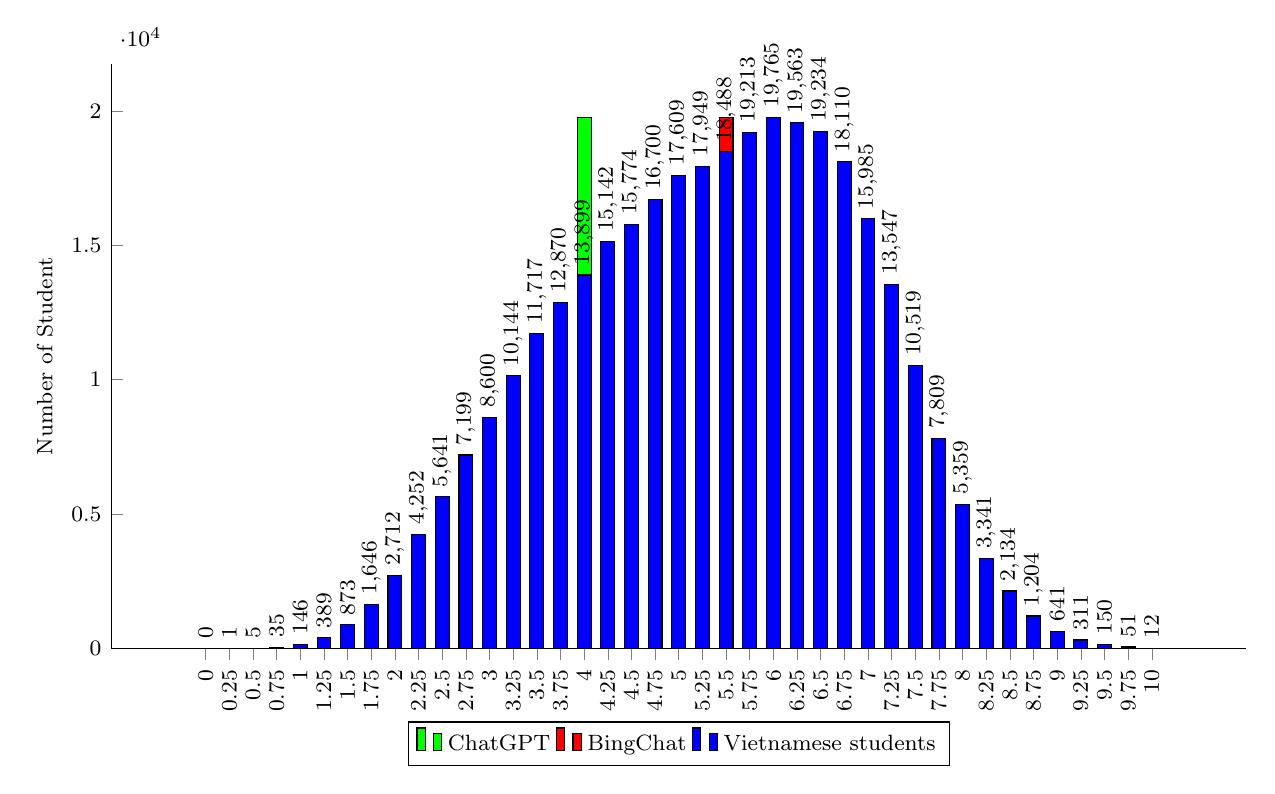
\begin{tikzpicture}
				\begin{axis}[
					legend style={at={(0.5,-0.125)}, 	
						anchor=north,legend columns=-1}, 
					symbolic x coords={
						0,
						0.25,
						0.5,
						0.75,
						1,
						1.25,
						1.5,
						1.75,
						2,
						2.25,
						2.5,
						2.75,
						3,
						3.25,
						3.5,
						3.75,
						4,
						4.25,
						4.5,
						4.75,
						5,
						5.25,
						5.5,
						5.75,
						6,
						6.25,
						6.5,
						6.75,
						7,
						7.25,
						7.5,
						7.75,
						8,
						8.25,
						8.5,
						8.75,
						9,
						9.25,
						9.5,
						9.75,
						10,	
					},
					%xtick=data,
					hide axis,
					ybar,
					bar width=5pt,
					ymin=0,
					%enlarge x limits,
					%nodes near coords,   
					every node near coord/.append style={rotate=90, anchor=west},
					width=\textwidth, 
					enlarge x limits={abs=0.5*\pgfplotbarwidth},
					height=9cm, 
					width=16cm,
					axis x line*=bottom, axis y line*=left
					]
					\addplot [fill=green] coordinates {
						(0,0)
					};
					\addplot [fill=red] coordinates {
						(5,0)
					};	
					\addplot [fill=blue] coordinates {
						(10,0)
					};	
					\legend{ChatGPT, BingChat,Vietnamese students}	
				\end{axis}
				
				\begin{axis}[
					symbolic x coords={
						0,
						0.25,
						0.5,
						0.75,
						1,
						1.25,
						1.5,
						1.75,
						2,
						2.25,
						2.5,
						2.75,
						3,
						3.25,
						3.5,
						3.75,
						4,
						4.25,
						4.5,
						4.75,
						5,
						5.25,
						5.5,
						5.75,
						6,
						6.25,
						6.5,
						6.75,
						7,
						7.25,
						7.5,
						7.75,
						8,
						8.25,
						8.5,
						8.75,
						9,
						9.25,
						9.5,
						9.75,
						10,	
					},
					%xtick=data,
					hide axis,
					x tick label style={rotate=90,anchor=east},
					ybar,
					bar width=5pt,
					ymin=0,
					%ymax=90000,
					%enlarge x limits,
					%nodes near coords,   
					every node near coord/.append style={rotate=90, anchor=west},
					width=\textwidth, 
					height=9cm, 
					width=16cm,
					axis x line*=bottom, axis y line*=left
					]
					\addplot [fill=green] coordinates {
						(0,0)
						(0.25,0)
						(0.5,0)
						(0.75,0)
						(1,0)
						(1.25,0)
						(1.5,0)
						(1.75,0)
						(2,0)
						(2.25,0)
						(2.5,0)
						(2.75,0)
						(3,0)
						(3.25,0)
						(3.5,0)
						(3.75,0)
						(4,30000)
						(4.25,0)
						(4.5,0)
						(4.75,0)
						(5,0)
						(5.25,0)
						(5.5,0)
						(5.75,0)
						(6,0)
						(6.25,0)
						(6.5,0)
						(6.75,0)
						(7,0)
						(7.25,0)
						(7.5,0)
						(7.75,0)
						(8,0)
						(8.25,0)
						(8.5,0)
						(8.75,0)
						(9,0)
						(9.25,0)
						(9.5,0)
						(9.75,0)
						(10,0)
					};	
				\end{axis}
				
				\begin{axis}[ 
					symbolic x coords={
						0,
						0.25,
						0.5,
						0.75,
						1,
						1.25,
						1.5,
						1.75,
						2,
						2.25,
						2.5,
						2.75,
						3,
						3.25,
						3.5,
						3.75,
						4,
						4.25,
						4.5,
						4.75,
						5,
						5.25,
						5.5,
						5.75,
						6,
						6.25,
						6.5,
						6.75,
						7,
						7.25,
						7.5,
						7.75,
						8,
						8.25,
						8.5,
						8.75,
						9,
						9.25,
						9.5,
						9.75,
						10,	
					},
					%xtick=data,
					hide axis,
					ybar,
					bar width=5pt,
					ymin=0,
					%ymax=90000,
					%enlarge x limits,
					%nodes near coords,   
					every node near coord/.append style={rotate=90, anchor=west},
					width=\textwidth, 
					height=9cm, 
					width=16cm,
					axis x line*=bottom, axis y line*=left
					]
					\addplot [fill=red] coordinates {
						(0,0)
						(0.25,0)
						(0.5,0)
						(0.75,0)
						(1,0)
						(1.25,0)
						(1.5,0)
						(1.75,0)
						(2,0)
						(2.25,0)
						(2.5,0)
						(2.75,0)
						(3,0)
						(3.25,0)
						(3.5,0)
						(3.75,0)
						(4,0)
						(4.25,0)
						(4.5,0)
						(4.75,0)
						(5,0)
						(5.25,0)
						(5.5,30000)
						(5.75,0)
						(6,0)
						(6.25,0)
						(6.5,0)
						(6.75,0)
						(7,0)
						(7.25,0)
						(7.5,0)
						(7.75,0)
						(8,0)
						(8.25,0)
						(8.5,0)
						(8.75,0)
						(9,0)
						(9.25,0)
						(9.5,0)
						(9.75,0)
						(10,0)
					};	
				\end{axis}
				\begin{axis}[
					ylabel={Number of Student},
					symbolic x coords={
						0,
						0.25,
						0.5,
						0.75,
						1,
						1.25,
						1.5,
						1.75,
						2,
						2.25,
						2.5,
						2.75,
						3,
						3.25,
						3.5,
						3.75,
						4,
						4.25,
						4.5,
						4.75,
						5,
						5.25,
						5.5,
						5.75,
						6,
						6.25,
						6.5,
						6.75,
						7,
						7.25,
						7.5,
						7.75,
						8,
						8.25,
						8.5,
						8.75,
						9,
						9.25,
						9.5,
						9.75,
						10,	
					},
					xtick=data,
					x tick label style={rotate=90,anchor=east},
					ybar,
					bar width=5pt,
					ymin=0,
					%enlarge x limits,
					nodes near coords,   
					every node near coord/.append style={rotate=90, anchor=west},
					width=\textwidth, 
					height=9cm, 
					width=16cm,
					axis x line*=bottom, axis y line*=left
					]
					\addplot [fill=blue] coordinates {
						(0,0)
						(0.25,1)
						(0.5,5)
						(0.75,35)
						(1,146)
						(1.25,389)
						(1.5,873)
						(1.75,1646)
						(2,2712)
						(2.25,4252)
						(2.5,5641)
						(2.75,7199)
						(3,8600)
						(3.25,10144)
						(3.5,11717)
						(3.75,12870)
						(4,13899)
						(4.25,15142)
						(4.5,15774)
						(4.75,16700)
						(5,17609)
						(5.25,17949)
						(5.5,18488)
						(5.75,19213)
						(6,19765)
						(6.25,19563)
						(6.5,19234)
						(6.75,18110)
						(7,15985)
						(7.25,13547)
						(7.5,10519)
						(7.75,7809)
						(8,5359)
						(8.25,3341)
						(8.5,2134)
						(8.75,1204)
						(9,641)
						(9.25,311)
						(9.5,150)
						(9.75,51)
						(10,12)
					};	
				\end{axis}
			\end{tikzpicture}

\end{document}